%-----------------------------------------------------------------------------------------
\clearpage
\section{Background Research}
%-----------------------------------------------------------------------------------------

In this section, a literature review is first introduced to present the most relevant works to this project. In the second part, previous systems in a similar project are introduced. The third part provides a detailed analysis of the data characteristics.

\subsection{Literature Review}

This section defines principles and techniques for data preprocessing and text data visualisation.

Text Visualisation Browser \cite{Kucher2014} is an online tool which provides the most comprehensive summary of published text visualisation \cite{Cao2016}. According to Text Visualisation Browser, from 1976 to 2017, there exist 400 published text visualisation papers in total, in which 396 publications are aimed to analyze text alignment. By searching 'Word', there shows 20 publications, and 'Translation' gets 16 results. Whereas when typing 'Frequency' and 'Weighting', each keyword gets one results. Also, keywords such as 'Machine learning, 'Data Mining', 'Natural Language Processing' got no publication collected. The results indicate that in text visualisation domain, most researchers focus on presenting alignment of texts. There are certain amounts of research focus on the topic such as 'word analysis' and 'translation', which is similar to this project. However, applying more specific techniques such as 'Natural Language Processing' haven't been applied in text visualisation widely.


\paragraph{Interactive Exploration of Versions across Multiple Documents}

\paragraph[]{}In the work of \emph{Interactive Exploration of Versions across Multiple Documents}, \cite{Jong2008} provide an interactive visualisation tool, MultiVersioner, to address the issues of comparing several versions of texts. The MultiVersioner enables users to search for items such as words, phrases and lines, along with the analysis of the frequency patterns of these items. In addition, methods such as colour-coded highlighting and overview are also rendered in this tool. Figure \ref{fig:multiVersioner} serves as an example of overview for many versions and documents in this software. In the overview, terms are denoted by blocks. If user mouses over a single block, a tooltip with the relevant sentence will be popped up.

\begin{figure}[H]
	\centering    
	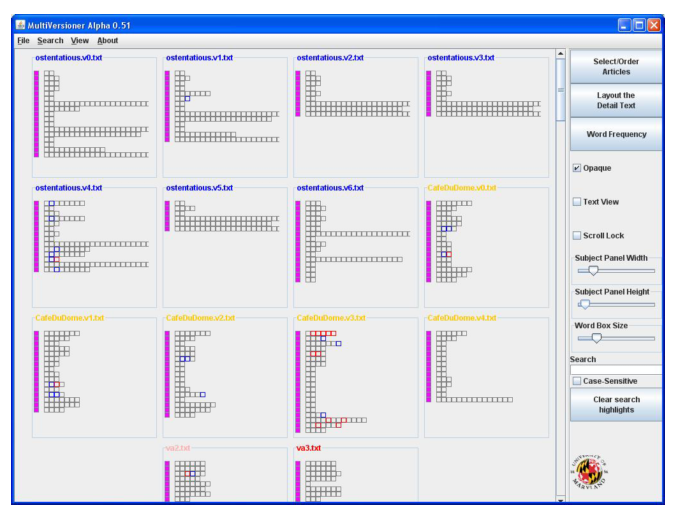
\includegraphics[scale=0.9]{Figs/MultiVersioner}\\[1ex]
	\caption{An overview of many versions and documents in MultiVersioner (\cite{Jong2008}).}
	\label{fig:multiVersioner}
\end{figure} 

The work of MultiVersioner allows users to compare multiple documents. Meanwhile, it provides a helpful feature to search for entities such as words and lines. Moreover, it can be served as a tool to analyse the frequency patterns of the words. However, there are only limited features provided in this software. Some helpful functions such as alignments between versions, or version turning on and off need to be explored.

\paragraph{Interactive Visual Alignment of Medieval Text Versions}
\paragraph[]{}

\cite{Stefan2017} discussed novel methods to compare text versions in the work \emph{Interactive Visual Alignment of Medieval Text Versions}. They provide a visual analytics system which enables computationally align complex textual differences such as orally inflected text. The data they deal with is a group of medieval poetries with complex text forms. Their works include three basic visualisations:

\begin{itemize}
	\item \textbf{A visualisation of text alignment} This is a visualisation in which highly unstable text versions are identified and aligned. This feature is accomplished applying parameter-driven approach. Moreover, a visual analytic process is rendered which accept tweaking parameters for iterative improvement of the alignment.
	\item \textbf{Multi-level alignment visualisation} In this view, various visualisations are presented which enables users to analyse texts alignments on different hierarchy levels.
	\item \textbf{Meso Reading} This is a visualisation to interpret texts in parallel. Similarly, the connections are demonstrated among text versions. This feature is considered as a novel feature which provides an intermediate perspective to display complex variance in texts.
	
	Figure \ref{fig:mesoReading} is an interpretation of this project. The screenshot in \cite{Stefan2017} displays different views of the distant reading, the meso reading, the close reading, and full-line matches. In part one, distant reading results of high similarity on words are displayed in the form of parallel lines. In addition, diagonal lines represent several repetitions. In part two, meso reading results are shown in the verse line 'Qui me dist que li ange sont'. In part three, a close reading feature is explored to show false positive alignment while part four are the matches for numerous full-line text.
	
	\begin{figure}[H]
		\centering    
		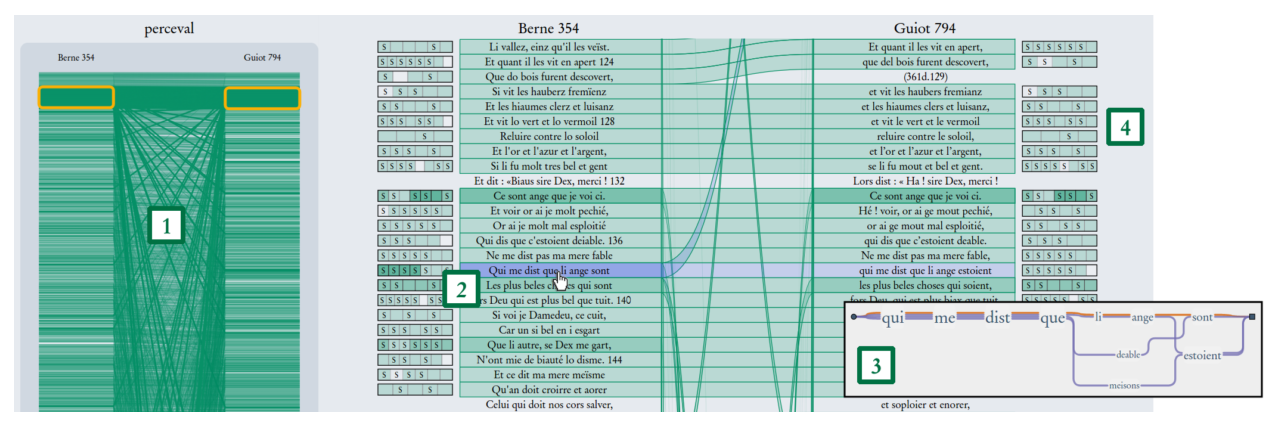
\includegraphics[scale=0.5]{Figs/Meso-Reading}\\[1ex]
		\caption{ (1) distant reading (2) meso reading (3) close reading (4) full-line matches (\cite{Stefan2017}).}
		\label{fig:mesoReading}
	\end{figure} 
	
	
\end{itemize}

However, this tool is more suitable for French context, which limited the rage of data text can be processed applying methods in this work.

\paragraph{Visualizations Translation Variation of Shakespeare's \emph{Othello}: A Survey of Text Visualisation and Analysis Tools}
\paragraph[]{} In their work \emph{Visualizations Translation Variation of Shakespeare's \emph{Othello}: A Survey of Text Visualisation and Analysis Tools}, \cite{Geng2011} developed a visualisation system which can be used to view and analyse variations between translation and based text. The data of this project is a collection of German translations of Shakespeare's \emph{Othello}. In this project, several techniques are applied to get an interactive visualisation system. These techniques include parallel coordinate, Tree-map, and DOI-tree. The tools which they developed provides features that enable users to brush words so that these words can be displayed in a parallel tag cloud. Figure \ref{fig:tagCloud} is a screen shot which illustrates the outcome of applying the TagCrowd feature into one of \emph{Othello} translation version. In this view, the stop words are identified and removed manually from the original text.

\begin{figure}[H]
	\centering    
	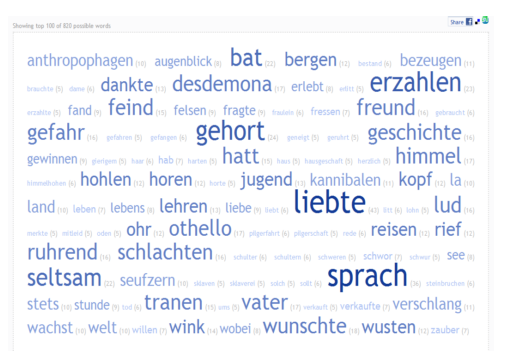
\includegraphics[scale=1]{Figs/Tagcloud}\\[1ex]
	\caption{The TagCrow (\cite{TagCrowd}) visualisation of a passage from \emph{Othello}.}
	\label{fig:tagCloud}
\end{figure} 

\paragraph{ShakerVis: Visual Analysis of Segment Variation of German Translations of Shakespeare’s \emph{Othello}}
\paragraph[]{} ShakerVis \cite{Geng2015} is a special visualisation tool which is designed to provide an interactive visualisation system to display version variations. In this system, \cite{Geng2015} applies following visualisation techniques:

\begin{itemize}
	\item \textbf{Parallel Coordinate View} provides outcomes by using Eddy value. The description of Eddy value can be seen in Previous System chapter.
	\item \textbf{Scatter Plot View} presents an average similarity value for each translation across multiple segments.
	\item \textbf{Term-document Frequency Heat Map} renders a way to analyse differences between pairs of versions in details, including a measurement of character-string similarities.
	
\end{itemize}

\subsection{Previous Systems}

The Version Variation Visualization (VVV) project was introduced by Dr Tom Cheesman from Modern Language Centre at Swansea University. It aims to create interactive data visualisation system to build cross-cultural exploration networks. The VVV project focus on developing digital tools which can help to compare and analyze different versions of translation \cite{Cheesman2012}. So far, the tools developed in the project is Ebla, Prism and ShakerVis. Ebla served as the corpus, is a software to stock the text data and detailed information about them. Prism provides the interface for separating texts into segments and processing the segments as alignment. Based on the idea of this two software, ShakerVis provides an interactive interface for visualizing the information of the translation versions \cite{Geng2015}.

There are three types of data visualisation in this project: Time-Map, Alignment Maps, Parallel view and Eddy and Viv view. 

\paragraph{Time-Map}
\paragraph[]{}

Figure \ref{fig:timeMap} supplies a screen shot of Time Map, which shows the location of the authors and the year of translation versions published. From this view, we can tell that some particular places such as Berlin and Dresden in which more authors were born this places and more translaitons versions were published from here. This can be deemed as that these two cities are popular places with large scale of city.

\begin{figure}[H] 
	\centering    
	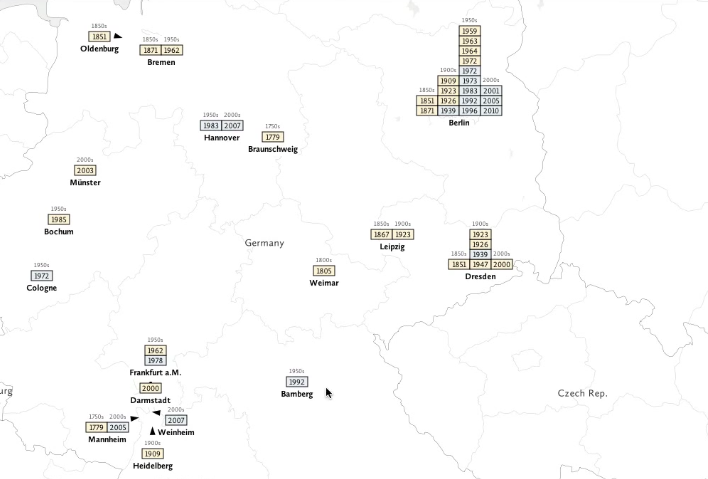
\includegraphics[scale=0.7]{Figs/Time-Map}\\[1ex]
	\caption{A demo screen shot for Time-Map (\cite{Cheesman2012}).}
	\label{fig:timeMap}
\end{figure} 

\paragraph{Alignment Map}
\paragraph[]{}

Figure \ref{fig:alignmentMap} exhibits a parallel visualisation which provides an alignment from the segments in th base texts to the translation versions. The yellow parts highlighted the whole segment selected while the blue line serves as the alignments. By comparing these texts, one can tell the general differences between the base text and translations. For example, if one segment of certain translation is longer than that of the base text, it is possible that a particular expression in German is appeared. 

\begin{figure}[H] 
	\centering    
	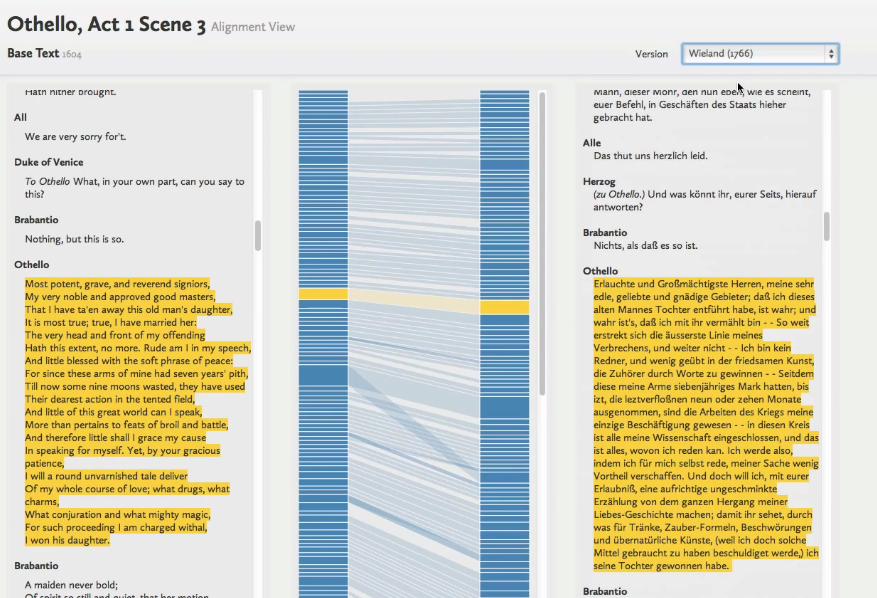
\includegraphics[scale=0.7]{Figs/Alignment-Map}\\[1ex]
	\caption{A screen shot of the demo of Alignment Maps (\cite{Cheesman2012}).}
	\label{fig:alignmentMap}
\end{figure} 

\paragraph{Parallel View}
\paragraph[]{}

Parallel View provides an explicit view between the base text and selected version. Figure \ref{fig:parallelView} shows a straightforward view of base text and selected translations. In this visualisation, segments are more explicit to find.

\begin{figure}[H] 
	\centering    
	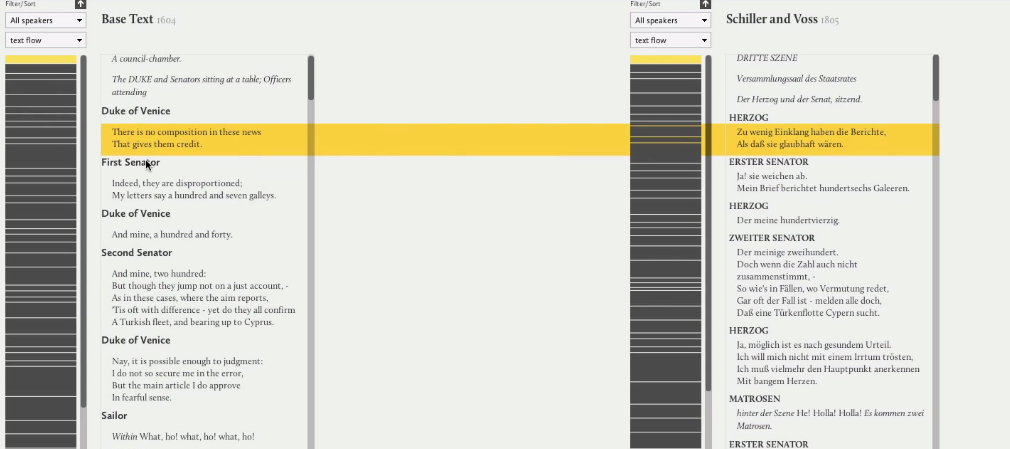
\includegraphics[scale=0.6]{Figs/Parallel-View}\\[1ex]
	\caption{A screen shot for the demo of Parallel View (\cite{Cheesman2012}).}
	\label{fig:parallelView}
\end{figure} 

\paragraph{Eddy and Viv View}
\paragraph[]{}

Eddy and Vis view enable researchers to understand more details of vocabulary. Figure \ref{fig:eddyVivView} demonstrates Eddy and Viv view, which provides more information of the translation comparison. From the sort bar, we can tell that there are four types can be visualized. Eddy value shows the variation of words used in the segment. Relatively, Viv value provides the changes or rivalries for some segments in translation. If we choose version name, segment length or reference date as the order of sorting, there will be other information on translation variations. Also, there are back-translation based on machine translation provided, which is another powerful function for comparing the text data.

\begin{figure}[H] 
	\centering    
	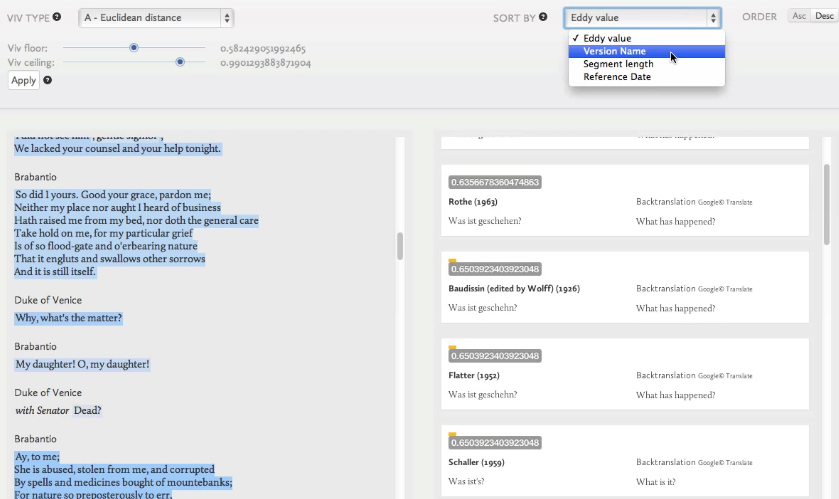
\includegraphics[scale=0.6]{Figs/Eddy-Viv-View}\\[1ex]
	\caption{A screen shot of Eddy and Vis view (\cite{Cheesman2012}).}
	\label{fig:eddyVivView}
\end{figure} 



